\documentclass[a4paper,12pt,oneside]{book}

%-------------------------------Start of the Preable------------------------------------------------
\usepackage[english]{babel}
\usepackage{blindtext}
%packagr for hyperlinks
\usepackage{hyperref}
\hypersetup{
    colorlinks=true,
    linkcolor=blue,
    filecolor=magenta,      
    urlcolor=cyan,
}

\urlstyle{same}
%use of package fancy header
\usepackage{fancyhdr}
\setlength\headheight{26pt}
\fancyhf{}
%\rhead{
\includegraphics[width=1cm]{logo}}
\lhead{\rightmark}
\rhead{
\includegraphics[width=1cm]{logo}}
\fancyfoot[RE, RO]{\thepage}
\fancyfoot[CE, CO]{\href{http://www.e-yantra.org}{www.e-yantra.org}}

\pagestyle{fancy}

%use of package for section title formatting
\usepackage{titlesec}
\titleformat{\chapter}
  {\Large\bfseries} % format
  {}                % label
  {0pt}             % sep
  {\huge}           % before-code
 
%use of package tcolorbox for colorful textbox
\usepackage[most]{tcolorbox}
\tcbset{colback=cyan!5!white,colframe=cyan!75!black,halign title = flush center}

\newtcolorbox{mybox}[1]{colback=cyan!5!white,
colframe=cyan!75!black,fonttitle=\bfseries,
title=\textbf{\Large{#1}}}

%use of package marginnote for notes in margin
\usepackage{marginnote}

%use of packgage watermark for pages
%\usepackage{draftwatermark}
%\SetWatermarkText{
\includegraphics{logo}}
\usepackage[scale=2,opacity=0.1,angle=0]{background}
\backgroundsetup{
contents={
\includegraphics{logo}}
}

%use of newcommand for keywords color
\usepackage{xcolor}
\newcommand{\keyword}[1]{\textcolor{red}{\textbf{#1}}}

%package for inserting pictures
\usepackage{graphicx}
\usepackage{float}
\usepackage{caption}
\usepackage{subcaption}

%package for highlighting
\usepackage{color,soul}

%new command for table
\newcommand{\head}[1]{\textnormal{\textbf{#1}}}


%----------------------End of the Preamble---------------------------------------


\begin{document}

%---------------------Title Page------------------------------------------------
\begin{titlepage}
\raggedright
{\Large eYSIP2018\\[1cm]}
{\Huge\scshape Flying Sensor Node \\[.1in]}
\vfill
\begin{flushright}
{\large \hspace{0.05cm} Intern : Abheet Verma \\}
{\large Intern \hspace{0.05cm} : Chirag Shah \\}
\hfill \linebreak
{\large Mentor : Simranjeet Singh \\}
{\large Mentor : Saurav Shandilya \\}
\hfill \linebreak
{\large Duration of Internship: $ 21/05/2018-06/07/2018 $ \\}
\end{flushright}

{\itshape 2018, e-Yantra Publication}
\end{titlepage}
%-------------------------------------------------------------------------------

\chapter[Project Tag]{Flying Sensor Node}
\section*{Abstract}

Drone and IoT are two emerging technologies having a plethora of applications. Through this project we aim to bridge these technologies to develop an indoor and outdoor environment monitoring system. A drone acts as a sensor node and flies across a room using way points predetermined by the user, collecting the temperature and humidity data using on-board sensors. The sensor data along with the location and time stamp are sent to central IoT server for data visualization and analytics.\\ \\ 
Different drones were used for indoor and outdoor environments to tackle the unique challenges faced in terms of mobility and localization in each environment. The concept of charging the drone through a landing deck was also explored in order to realize the potential of Flying Sensor Node in real world applications. The necessity of this system can be found in places such as greenhouses, where the environment needs to be monitored to schedule tasks such as irrigation, fertilizing etc. \\ \\
A wireless sensor network if installed in such an area would require a huge number of nodes. Hence, resulting in increased maintenance effort and cost. Sensor nodes are static and hence can only give feedback at fixed points in the monitoring area, leading to loss in critical information. If considering a greenhouse a leakage in the irrigation system in a place not monitored by a sensor node will go undetected but a flying sensor node will be able to detect parameters at every point in its path.\\ \\
The goal of this project was not only to get the flying sensor node's data but to also make it accessible to the user in a manner which is simple and intuitive. In order to achieve this goal an Internet of Things dashboard was built which allows the user to visualize sensor data and also control some basic functionalities of the drone. The platforms were different for both indoor and outdoor flying sensor nodes, according to the capabilities of each drone. For example the dashboard for the outdoor flying sensor node has a live video stream and live tracking on maps whereas the indoor flying sensor node has control commands on the server.

\subsection*{Completion status}
\subsubsection{Indoor Flying Sensor Node Tasks} 

\begin{itemize}
\item Pluto X on-board sensor and peripheral interfacing using existing APIs.
\item STM32f303CB peripheral interfacing using standard peripheral libraries.
\item AR Drone navigation in Gazebo simulation for both Whycon and GPS.
\item AR Drone communication in Gazebo simulation for IMU values.
\item IoT Server for sensor data visualisation and live tracking was created on the control station.
\item Establish communication between Drone and IoT Platform in simulation and reality.
\item Decawave UWB tag and anchor hardware setup and configuration.
\item UWB tag interfacing on Pluto X.
\item Pluto X location co-ordinates transmission and reception using Multi Wii Serial Protocol.
\item Complementary Filter design for localization data (Needs Improvement).
\item Payload Testing of Pluto X.
\item Waypoint planning and navigation with data logging using UWB and Whycon.
\item Landing of Pluto X on designated charging area. 
\end{itemize}

\subsubsection{Outdoor Flying Sensor Node Tasks} 

\begin{itemize}
\item Quadcopter assembly and RC remote testing.
\item Pixhawk setup and configuration using Mission Planner and Q Ground Control was attempted.
\item Pixhawk control using mavros, dronekit and companion computer was attempted.
\item Navio 2 setup for quadcopter was done on RPi.
\item Quadcopter configuration and calibration was done using Mission Planner.
\item IoT Server for sensor data visualisation, live tracking and video streaming was created on the RPi.
\item Location logging using GPS was implemented.
\item Temperature and humidity value from DHT-22 is communicated to the flight controller and is logged.
\item Mounting structure for Sensor node was designed.
\item Battery consumption was analyzed and appropriate power source was selected.
\item Fail safes like Geofence,3D Fix and other Prearm Checks like Barometer,Gyro etc were removed to enable indoor testing.
\item Stabilize mode of operation was tested indoors using RC transmitter.
\end{itemize}

\section{Hardware parts}

\subsubsection{Pluto X } 

\begin{itemize}
  \item Purpose : Indoor Drone based on STM32f303CB
  \item Vendor  : Drona Aviation 
 \end{itemize}
 
 \subsubsection{RPI} 

\begin{itemize}
  \item Purpose : RPI 3B is the processing unit for the outdoor quadcopter when using Navio 2. 
  \item Product Link : \href{https://www.raspberrypi.org/products/raspberry-pi-3-model-b/}{RPI 3B} 
  \item Datasheet : \href{https://cdn.sparkfun.com/datasheets/Dev/RaspberryPi/2020826.pdf}{RPI 3B Datasheet} 
 \end{itemize}
 
 \subsubsection{Arduino Nano } 

\begin{itemize}
  \item Purpose : Arduino Nano is used as sensor node.
  \item Product Link : \href{https://robu.in/product/arduino-nano-v3-0-ch340-chip-mini-usb-cable/?gclid=CjwKCAjw4PHZBRA-EiwAAas4ZnkY1Uyx1regBeSCiAQphWNPrAL1DfNjwFlLTFBN2IuJMkXe9YMaixoCQcsQAvD_BwE}{Arduino Nano} 
  \item Datasheet : \href{https://www.arduino.cc/en/uploads/Main/ArduinoNanoManual23.pdf}{Arduino Nano Datasheet} 
 \end{itemize}

 \subsubsection{Navio 2 } 

\begin{itemize}
  \item Purpose : Navio 2 is an autopilot hat for RPi that has all the sensors and controllers onboard like Dual IMU,Barometer,GNSS receiver,RC I/O co-processor etc. 
  \item Product Link : \href{https://store.emlid.com/product/navio2/}{Navio 2} 
  \item Product Brief : \href{https://docs.emlid.com/navio2/}{Navio 2 Documentation} 
 \end{itemize}
 
 \subsubsection{Decawave DWM1001 } 

\begin{itemize}
  \item Purpose :Indoor Localization
  \item Product Link : \href{https://www.findchips.com/search/DWM1001?gclid=CjwKCAjw4PHZBRA-EiwAAas4ZtTtjHXX9dnmI99yqhUIe2f_LFBmznETxFEPqzojVR2hLfT5Xpz6JRoCmh8QAvD_BwE&gclsrc=aw.ds}{DWM 1001} 
  \item Product Brief : \href{https://www.decawave.com/products/dwm1001-module}{DWM 1001 Resources} 
 \end{itemize}
 
 \subsubsection{LiPo Battery 6200 mAh, 40C \& 11.1 V } 

\begin{itemize}
  \item Purpose : Powering the quadcopter.
  \item Product Link : \href{https://robu.in/product/orange-11-1v-6200mah-3s-40c-lipo-battery-pack-xt60-connector/}{Orange Battery} 
  \item Product Brief : \href{https://robu.in/product/orange-11-1v-6200mah-3s-40c-lipo-battery-pack-xt60-connector/}{Orange Battery Specifications} 
 \end{itemize}
 
  \subsubsection{Pixhawk} 
\begin{itemize}
  \item Purpose : Flight controller
  \item Product Link : \href{https://robokits.co.in/drones-quad-hexa-octa-fpv/flight-controllers/pixhawk-px4-2.4.8-32bit-flight-controller-with-imp.-accessories}{Pixhawk} 
  \item Product Brief : \href{https://pixhawk.org/}{Pixhawk Resources} 
 \end{itemize}
 
\subsubsection{Telemetry Radio 433MHz for Navio 2 } 

\begin{itemize}
  \item Purpose : Communication between ground control station and quadcopter. 
  \item Product Link : \href{https://store.mrobotics.io/mRo-SiK-Telemetry-Radio-V2-433Mhz-p/mro-433sikv2-mr.htm}{Mrobotics Telemetry Module} 
 \end{itemize}

\subsubsection{Telemetry Radio 433MHz for Pixhawk } 

\begin{itemize}
  \item Purpose : Communication between ground control station and quadcopter. 
  \item Product Link : \href{https://robokits.co.in/drones-quad-hexa-octa-fpv/fpv-video-telemetry-osd/433mhz-telemetry-module-pair-for-pixhawk-and-apm-100mw-2km-range}{Pixhawk Compatible Telemetry Module} 
   \end{itemize}
 
 \subsubsection{DHT-22} 

\begin{itemize}
  \item Purpose : Sensor for obtaining temperature and humidity data. 
  \item Product Link : \href{https://www.amazon.in/Generic-Digital-Temperature-Humidity-Sensor/dp/B00O8RIYYU}{DHT-22} 
  \item Product Brief : \href{https://www.sparkfun.com/datasheets/Sensors/Temperature/DHT22.pdf}{DHT-22 Datasheet} 
 \end{itemize}
 
  \subsubsection{Brushless Motor Speed Controller ESC 30A} 

\begin{itemize}
  \item Purpose : Electronic speed controller for BLDCs.
  \item Product Link : \href{https://robokits.co.in/quadrotors-hexarotors-drones/brushless-motors-esc/brushless-motor-speed-controller-esc-30a/}{ESC Specifications} 
 \end{itemize}

\subsubsection{RC Brushless Motor 2212 1000KV With Soldered Banana Connector} 

\begin{itemize}
  \item Purpose : BLDCs with propellers to provide motion to the quadcopter. Various movements are possible by varying the direction of rotation of propellers \& by altering the speed of the motors.

 
  \item Product Link : \href{https://robokits.co.in/quadrotors-hexarotors-drones/brushless-motors-esc/brushless-motor-speed-controller-esc-30a/}{BLDC Specifications} 
 \end{itemize}

\section{Software used}

 \subsection{Indoor}
 \begin{itemize}
  \item Java
  
  For Windows:\href{http://www.oracle.com/technetwork/java/javase/downloads/jdk8-downloads-2133151.html}{Link}\\
  For Ubuntu:\href{http://tipsonubuntu.com/2016/07/31/install-oracle-java-8-9-ubuntu-16-04-linux-mint-18/}{Link}
  
  Use Java 8 only as it is required for Cygnus.

  \item Cygnus IDE
  
  This integrated developement environment is necessary for flashing code to the pluto drone.Install cygnus from \href{https://drive.google.com/drive/folders/12yho1OL4OuOJdStSYlG2r4aEH-reXx16}{here}.Follow the \href{https://github.com/eYSIP-2018/Flying-Sensor-Node/wiki/Setting-Up-Cygnus}{instructions} to setup Cygnus on you system.Enjoy coding!!!!
  
  \item ROS(Indigo)
  
  Robot Operating System (ROS) is robotics middleware (i.e. collection of software frameworks for robot software development).Ros is required for interfacing Pluto and PlutoX.To know more about ROS visit \href{https://en.wikipedia.org/wiki/Robot_Operating_System}{here}.
  
  The main ROS client libraries (C++ and Python) are geared toward a Unix-like system, primarily
because of their dependence on large collections of open-source software. Hence these client libraries
require Linux operating system.\\
You \textbf{must} install the \textbf{ROS-Indigo in Ubuntu 14.04} on your PC/Laptop.

	Follow the installation instructions from \href{http://wiki.ros.org/indigo/Installation/Ubuntu}{here}.
   
   \item pluto\_drone
   
   Metapackage to control the plutodrone via services and topics. This package establishes a connection between laptop and the ESP module on the drone using a socket. Thereby using MSP protocol we can send instructions to the drone and receive data from onboard and external sensors. \href{http://wiki.ros.org/pluto_drone}{wiki} 
   
   
   \item Roslibjs
   
   Roslibjs is the core JavaScript library for interacting with ROS from the browser. It uses WebSockets to connect with rosbridge and provides publishing, subscribing, service calls.\\ The topics and services are used in the form of JSON. A connection string is used to establish a connection and then get access to the topics.\\
   Download link:
   \href{https://static.robotwebtools.org/roslibjs/current/roslib.min.js}{min}
   ::
   \href{https://static.robotwebtools.org/roslibjs/current/roslib.js}{full}
   Source:\href{https://github.com/RobotWebTools/roslibjs}{Github}
   Wiki:\href{http://www.ros.org/wiki/roslibjs/}{Roslibjs}\\
   
  \item Rosbridge\_suite
  
  Rosbridge provides a JSON API to ROS functionality for non-ROS programs. There are a variety of front ends that interface with rosbridge, including a WebSocket server for web browsers to interact with.
  \\\\
  Rosbridge suite allows access to the topics and services on the server.Hence topics can be subscribed and published upon to give commands to the robot.\\ For installation visit this \href{http://wiki.ros.org/rosbridge_suite}{link}.
 \end{itemize} 
  \begin{figure}[H]
  \centering
  \includegraphics[width=12cm, height=6cm]{server.png}
  \caption{Server for indoor drone}
  \end{figure}
  
  \subsection{Outdoor}
  \begin{itemize}
  \item Ground Control Station
  
  A ground control station (GCS) is a land-based control centre that provides the facilities for human control of Unmanned Aerial Vehicles (UAVs or "drones").\\ A ground control station helps in sending mission details,setting essential parameters,configuring the sensors,getting real time values of sensors etc.
  
  You may install one the below GCS:\\ \\
  Mission Planner::\href{http://ardupilot.org/planner/docs/common-install-mission-planner.html}{Link}(only for Windows)\\
  QGroundControl::\href{https://docs.qgroundcontrol.com/en/getting_started/download_and_install.html}{Link}
  
  \item Python 
  
  Python examples were available for Raspberry Pi in the documentation for navio 2. The GPS example was used to obtain latitude, longitude and fix status. Python was also used for obtaining sensor data through USB port from the arduino nano (Serial library was used in this case). The server was written using flask which again is based on python. Socket programming was also implemented in the flask server to update position of drone in the background. Also python was used to fetch and update data in the Sqlite3 database   \\ \\
  We used Python 2.7 for this project.
  \textbf{Always use same python version for every library as it may cause errrors}.\\
  For installation visit \href{https://www.python.org/getit/}{here}.
  
  \item Emlid Image for Raspberry Pi
  
  Raspberry Pi was flashed with a custom image of raspbian that comes with pre installed Ardupilot, Ros and other necessary packages required for automated vehicles(Plane,Rover,Copter). The image does not have a GUI and should be used by connecting through SSH. Reconfiguring the image to enable GUI is not recommended as certain issues in the working were observed such as git-hub commands not working and autopilot parameters not updating. \\Download the \href{http://files.emlid.com/images/emlid-raspbian-20180525.img.xz}{image} and flash it on a memory card using \href{https://etcher.io/}{Etcher}
  \\
  Run and install Etcher using admin rights.\\Select the archive with Image and drive location.\\Click Flash!!.This may take a few minutes.
  
  \item Motion
  
  Motion is a highly configurable program that monitors video signals from many types of cameras. It was used for displaying live video feed on the web server coming from RPi Camera mounted on the Raspberry Pi. Setting it up  on raspberry pi can be understood from this \href{https://pimylifeup.com/raspberry-pi-webcam-server/}{link}. If the video doesn't start as soon as the server starts and a gray screen is visible visit this \href{https://raspberrypi.stackexchange.com/questions/60669/unable-to-open-video-device
}{discussion}
  
 
  \item Flask
  
  Flask is a micro web framework written in Python. It is classified as a micro-framework because it does not require particular tools or libraries. It is also very intuitive to use. Also as it is based in python, it is compatible with examples provided by emlid for navio 2. Read more about flask from \href{http://flask.pocoo.org/docs/}{here}.
  
  \item Sqlite 3
  
	Sqlite 3 is the database which was selected to log data locally. Follow this 
  \href{http://www.instructables.com/id/From-Data-to-Graph-a-Web-Jorney-With-Flask-and-SQL
}{tutorial} to understand setting up an IoT server using flask and displaying data logged in an Sqlite 3 database. 
  \begin{figure}[H]
  \centering
  \includegraphics[width=8cm, height=6cm]{home.png}
  \caption{Home page}
  \end{figure}
  \begin{figure}[H]
  \centering
  \includegraphics[width=9cm, height=6cm]{track.png}
  \caption{Live tracking}
  \end{figure}
  \begin{figure}[H]
  \centering
  \includegraphics[width=11cm, height=6cm]{picam.png}
  \caption{Live Video Feed}
  \end{figure}
  \begin{figure}[H]
  \centering
  \includegraphics[width=11cm, height=6cm]{sensor.png}
  \caption{Sensor data}
  \end{figure}
\end{itemize}

\section{Assembly of hardware}
The assembly for both indoor and outdoor drones is explained in this section. 

\subsection*{Indoor Flying Sensor Node} 

\subsubsection*{DWM1001 Module Setup}
\begin{itemize}
  \item One module is used as a tag on the drone.Connection between tag and PlutoX is shown as shown in the Figure-1.6 below.
  \begin{figure}[H]
 \centering
 \includegraphics[width=13cm, height=6cm]{Pinout_DWM.png}
 \caption{Pinout of DWM Module}
 \end{figure}
  \item Four modules are used as anchors on the wall.Each one of them requires a power source of 3.3V.

  \item The modules are configured using the official \href{https://play.google.com/store/apps/details?id=com.decawave.argomanager}{Decawave Android App}
  \item The instructions for the same are explained in the android application in great detail. 
 \end{itemize}

\subsubsection*{Pluto X}
\begin{itemize}
  \item The pin mapping of the shield with respect to the STM32f303CB micro-controller on Pluto X is as shown in the table in the Figure 1.7. 
  \begin{figure}[H]
  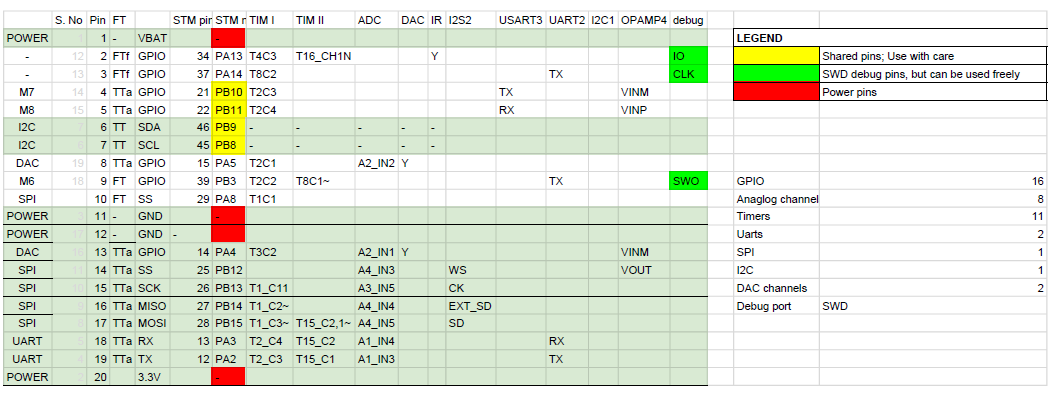
\includegraphics[width=15cm, height=6cm]{pinout.PNG}
  \caption{Pin Mapping of Pluto X Shield }
  \end{figure}
  \item After attaching the tag on the gpio shield of Pluto X, place the shield on the Pluto X as shown in the Figure 1.8 and 1.9.
  
  \begin{figure}[H]
\centering
\begin{subfigure}{.48\textwidth}
  \centering
  \includegraphics[width=.8\linewidth]{ShieldTop.jpg}
  \caption{Top View of Pluto-X shield}
  \label{fig:sub1}
\end{subfigure}%
\begin{subfigure}{.5\textwidth}
  \centering
  \includegraphics[width=.8\linewidth]{shield.jpg}
  \caption{Back Side view of Pluto-X shield}
  \label{fig:sub2}
\end{subfigure}
\caption{Pluto X Shield}
\label{fig:test}
\end{figure}
  
  \begin{figure}[H]
\centering
\begin{subfigure}{.6\textwidth}
  \centering
  \includegraphics[width=.8\linewidth]{PlutoX_without_shield.jpg}
  \caption{Pluto X without shield}
  \label{fig:sub1}
\end{subfigure}%
\begin{subfigure}{.5\textwidth}
  \centering
  \includegraphics[width=.8\linewidth]{Pluto_w_shield.jpg}
  \caption{Pluto X with shield}
  \label{fig:sub2}
\end{subfigure}
\caption{Pluto X Shield Setup}
\label{fig:test}
\end{figure}
   
\item A whycon marker is also added on top of the Pluto X as shown in the Figure 1.10 below to enable landing on charging area using an overhead camera. \\ \\
\begin{figure}[H]
\centering
\includegraphics[width=9cm, height=9cm]{whycon.jpg}
\caption{PlutoX with Whycon Marker Mounted}
\end{figure}
\end{itemize}

\subsection*{Outdoor Flying Sensor Node}
\subsubsection*{Auto Pilot Assembly}
\begin{itemize}
\item Raspberry Pi, Navio 2, GPS antenna, Telemetry trans-receiver, battery monitor, remote receiver through PPM encoder and electronic speed controller inputs are connected as shown \href{https://docs.emlid.com/navio2/ardupilot/hardware-setup/}{here} \\ \\
Note: The PPM encoder allows to encode up to 8 PWM (pulse width modulated) signals into one PPM (pulse position modulation) signal. 
\item The other parts of the drone such as motors and propellers are assembled in accordance to this \href{http://ardupilot.org/copter/docs/connect-escs-and-motors.html}{guide} 
\item A three cell 11.1V, 6200mAh, 40C lithium polymer battery is used to power the drone
\item The completely assembled quadcopter is as shown in the Figure 1.11 .
\begin{figure}[H]
\centering
\includegraphics[width=9cm, height=9cm]{big_drone.jpg}
\caption{Outdoor Drone/Quadcopter}
\end{figure}
\item The sensor node comprising of the arduino nano, DHT-22 and USB connector is as shown in the Figure 1.12.

\begin{figure}[H]
\centering
\begin{subfigure}{.6\textwidth}
  \centering
  \includegraphics[width=.8\linewidth]{sensor_SV.jpg}
  \caption{Sensor Node Side View}
  \label{fig:sub11}
\end{subfigure}%
\begin{subfigure}{.6\textwidth}
  \centering
  \includegraphics[width=.8\linewidth]{sensor_top.jpg}
  \caption{Sensor node top View}
  \label{fig:sub21}
\end{subfigure}
\caption{Sensor Node Module}
\label{fig:test1}
\end{figure}
\item The sensor node needs to be plugged in any of the USB ports of the raspberry pi on the drone.
\end{itemize}

\section{Software and Code}
\href{https://github.com/eYSIP-2018/Flying-Sensor-Node/}{Github link} for the repository of code

\subsection*{Outdoor}
\begin{itemize}
\item \textbf{Arduino Code} - Contains code to interface DHT-22 using arduino nano on a Raspberry PI.
\item \textbf{Drone-Server} - Contains server and related files for drone and copy the folder on Raspberry PI.
\item \textbf{Ardupilot Setup} - \href{https://docs.emlid.com/navio2/}{link}

\end{itemize}

\subsection*{Indoor}
\begin{itemize}
\item \textbf{Documents} - Contains API for interfacing PlutoX board.
\item \textbf{Codes} - Contains testing codes for PlutoX and RF.
\item \textbf{Pluto-X Navigation-Whycon,Final,Navigation} - Different Navigation scripts for PlutoX
\item \textbf{PlutoX Firmware} - Firmware Changes for MSP protocol
\item \textbf{Server} - Establishing server for logging data and controlling drone remotely
\item \textbf{pluto\_drone} - Contains changes in navigation packages 
\end{itemize}


\subsection*{Use and Demo}
\subsubsection*{Outdoor}
\begin{itemize}
\item After setting up the raspberry with the custom image and configuring the quadcopter using mission planner do the following :-
\item \textbf{Step 1} - Change directory to Drone-Server
\item \textbf{Step 2} - Run command "sudo modprobe bcm2835-v4l2" to get video on web server.
\item \textbf{Step 3} - Run command "sudo python SensorLog.py" to get real time sensor data i.e. temperature and humidity
\item \textbf{Step 4} - Run command "sudo python GPS.py" to get real time sensor data i.e. GPS (only if the drone is outdoors)
\item \textbf{Step 5} - Run command "sudo python app.py" to start the server
\item \textbf{Step 6} - If the IP address of the raspberry pi is 192.168.43.238 open a browser on a device connected to the network and enter the URL 192.168.43.238:5010 to get access to the IoT platform.

\end{itemize}

\subsection*{Indoor}
After setting the DWM1001 module,whycon on the drone and the overhead camera follow the below steps.
\begin{itemize}
\item \textbf{Step 1} - Make changes to the serial\_msp.cpp and flash the firmware.
\item \textbf{Step 2} - Add changed files to pluto\_drone metapackage
\begin{itemize}
\item To add your own MSP headers first define it in the firmware in the serial\_msp.cpp file
\item Add the new MSP header in the service request.
\item Receive the data in global declared parameters in the \\Plutoservice.srv file
\end{itemize}

\item \textbf{Step 3} - Run the data\_via\_rosservice.py file to get coordinates and other data
\item \textbf{Step 4} - Run the drone\_comb.launch file and on another terminal run the navigation script.
\item \textbf{Step 5} - Run the rosbridge\_websocket launch and open comm.html in browser to control the drone and get data
\item \textbf{PS} - Play with the code to understand it better.
\end{itemize}

\href{https://www.youtube.com/watch?v=DnNQvGCwf-I}{Youtube Link} of demonstration video 

\section{Future Work}
\subsection{Outdoor}
\begin{itemize}
\item Manual and Autonomous testing of drone in outdoor environment using Ground Control Station. 
\item Full fledged IOT server for large scale use using internet.
\item Buildng Charging Dock for the drone.
\item Using Dronekit and similar libraries for controlling drone using server.
\end{itemize}
\subsection{Indoor}
\begin{itemize}
\item Building a Charging Dock for PlutoX.
\item External Sensor(Temperature,Humidity) Interfacing for PlutoX.
\item Designing a better noise reduction filter so that navigation is much smoother.
\item On-board Computing of path to reduce latency and improve performance.
\end{itemize}

\section{Bug report and Challenges}
\subsection{Outdoor}
\begin{itemize}
\item No heartbeat received from the Flight Controller Unit. Check if the correct mode of connection is selected and the  address(UDP,TCP/IP) is correct. Also check the telemetry module for any damage on both transmitter and receiver end.
\item Arming the quadcopter without GPS fix is generally not permissible but by changing failsafe parameters this can be bypassed.
\item Bad logging error due to SD card. Try formatting the SD card again.Make sure to select FAT32 as the memory allocation type.
\item Telemetery issues with Pixhawk flight controller. Check the telemetry module for any damage on both transmitter and receiver end.
\end{itemize}
\subsection{Indoor}
\begin{itemize}
\item Understanding the firmware of Pluto X. The firmware itself contains huge amount of code and to understand the flow of code was a little difficult.A more clear reference can be taken from the Cleanflight repository on github.
\item Reconfiguring the firmware to accept the coordinate values coming from DWM1001. It was done using existing apis mentioned as shown by Drona Aviation team. .
\item Understanding Multi Wii Serial Protocol of data transfer from drone to control station and vice versa. The protocol was studied using on-line resources and wiki page mentioned in Bibliography.
\item Reconfiguring the ROS communication package for PlutoX 'plutodrone' to accept new MSP headers.
\item Designing a filter to reduce noise in the coordinates.A complimentary filter fusing raw roll,pitch values with the coordinates was tried but a better filter can be used to make navigation smoother.
\item Navigating drone using PID and then switching dynamically between Whycon marker and Ultra Wide Band for better navigation.
\item Fine tuning of PID for smooth control of drone.
\item External sensor i.e. DHT-22 interfacing was attempted but was later neglected for the following reasons :-
\begin{itemize}
\item The payload i.e.the RFID tag, itself was leading to increased strain on the drone, and incorporating the sensor on the drone increases the weight further which lead to difficulty in the flight of the drone. (Reduced battery life and difficulty in taking off)
\item The DHT-22 is a sensor based on one wire protocol, and libraries and documentation for it are not readily available for ARM STM32f303CB. Also making changes in the firmware for the same, were attempted in the initial stage but led to random behavior of the drone. The source of random behavior was due to mistakes in the firmware by Drona Aviation which were later rectified. But the sensor interfacing plan was dropped due to the increased payload mentioned earlier.
\item On-board temperature sensor was later used to do the environment monitoring, but this data was inaccurate due to heat dissipation of on-board components. 
\end{itemize}
\end{itemize}

\begin{thebibliography}{li}
\bibitem{ros1}
Mastering ROS for Robotics Programming - Lentin Joseph
\bibitem{ros2}
Ros tutorials-
\href{http://wiki.ros.org/ROS/Tutorials}{Link}
\bibitem{ros3}
Programming Robots with ROS: A Practical Introduction to the Robot
Operating - Brian Gerkey, Morgan L. Quigley, and William D. Smart
\bibitem{cheat}
\href{http://www.tedusar.eu/files/summerschool2013/ROScheatsheet.pdf}{ROS cheatsheet}
\bibitem{navio}
Navio Documentation-\href{https://docs.emlid.com/navio2/}{link}
\bibitem{linux}
Linux-\href{https://ryanstutorials.net/linuxtutorial/}{Documentation}
\bibitem{python}
Python-\href{https://www.tutorialspoint.com/python/}{Documentation}
\bibitem{msp}
Multi Wii Serial Protocol-\href{http://www.multiwii.com/wiki/index.php?title=Multiwii_Serial_Protocol}{link}
\bibitem{navio2git}
Navio2 drivers-\href{https://github.com/emlid/Navio2}{Github}
\end{thebibliography}


\end{document}


